\message{ !name(report.tex)}\documentclass[two column]{article}
\usepackage[utf8]{inputenc}

\usepackage{amsmath,amsthm,amssymb}

\usepackage{subcaption}
\usepackage{graphicx}

\graphicspath{{./../images/}}

\usepackage{listings}


\usepackage{color}

\definecolor{gray}{rgb}{0.5,0.5,0.5}
\definecolor{orange}{rgb}{0.8,0,0}

\lstdefinestyle{ccode}{
  belowcaptionskip=1\baselineskip,
  breaklines=true,
  frame=L,
  xleftmargin=\parindent,
  language=C,
  showstringspaces=false,
  basicstyle=\footnotesize\ttfamily,
  keywordstyle=\bfseries\color{green},
  commentstyle=\color{gray},
  identifierstyle=\color{blue},
  stringstyle=\color{orange},
}

\def\listingsfont{\ttfamily} 
\def\listingsfontinline{\ttfamily}

\title{Report for computer exercise 1 - Filter in MPI}
\author{Anton Karlsson\\antka388\\931217-7117}
\date{}
\begin{document}

\message{ !name(report.tex) !offset(54) }
\begin{figure}[h]
  \centering
  \begin{subfigure}{0.3\textwidth}
    \includegraphics[width=\textwidth]{im1.png}
    \caption{Before filtering.}
  \end{subfigure}
  ~%
  \begin{subfigure}{0.3\textwidth}
    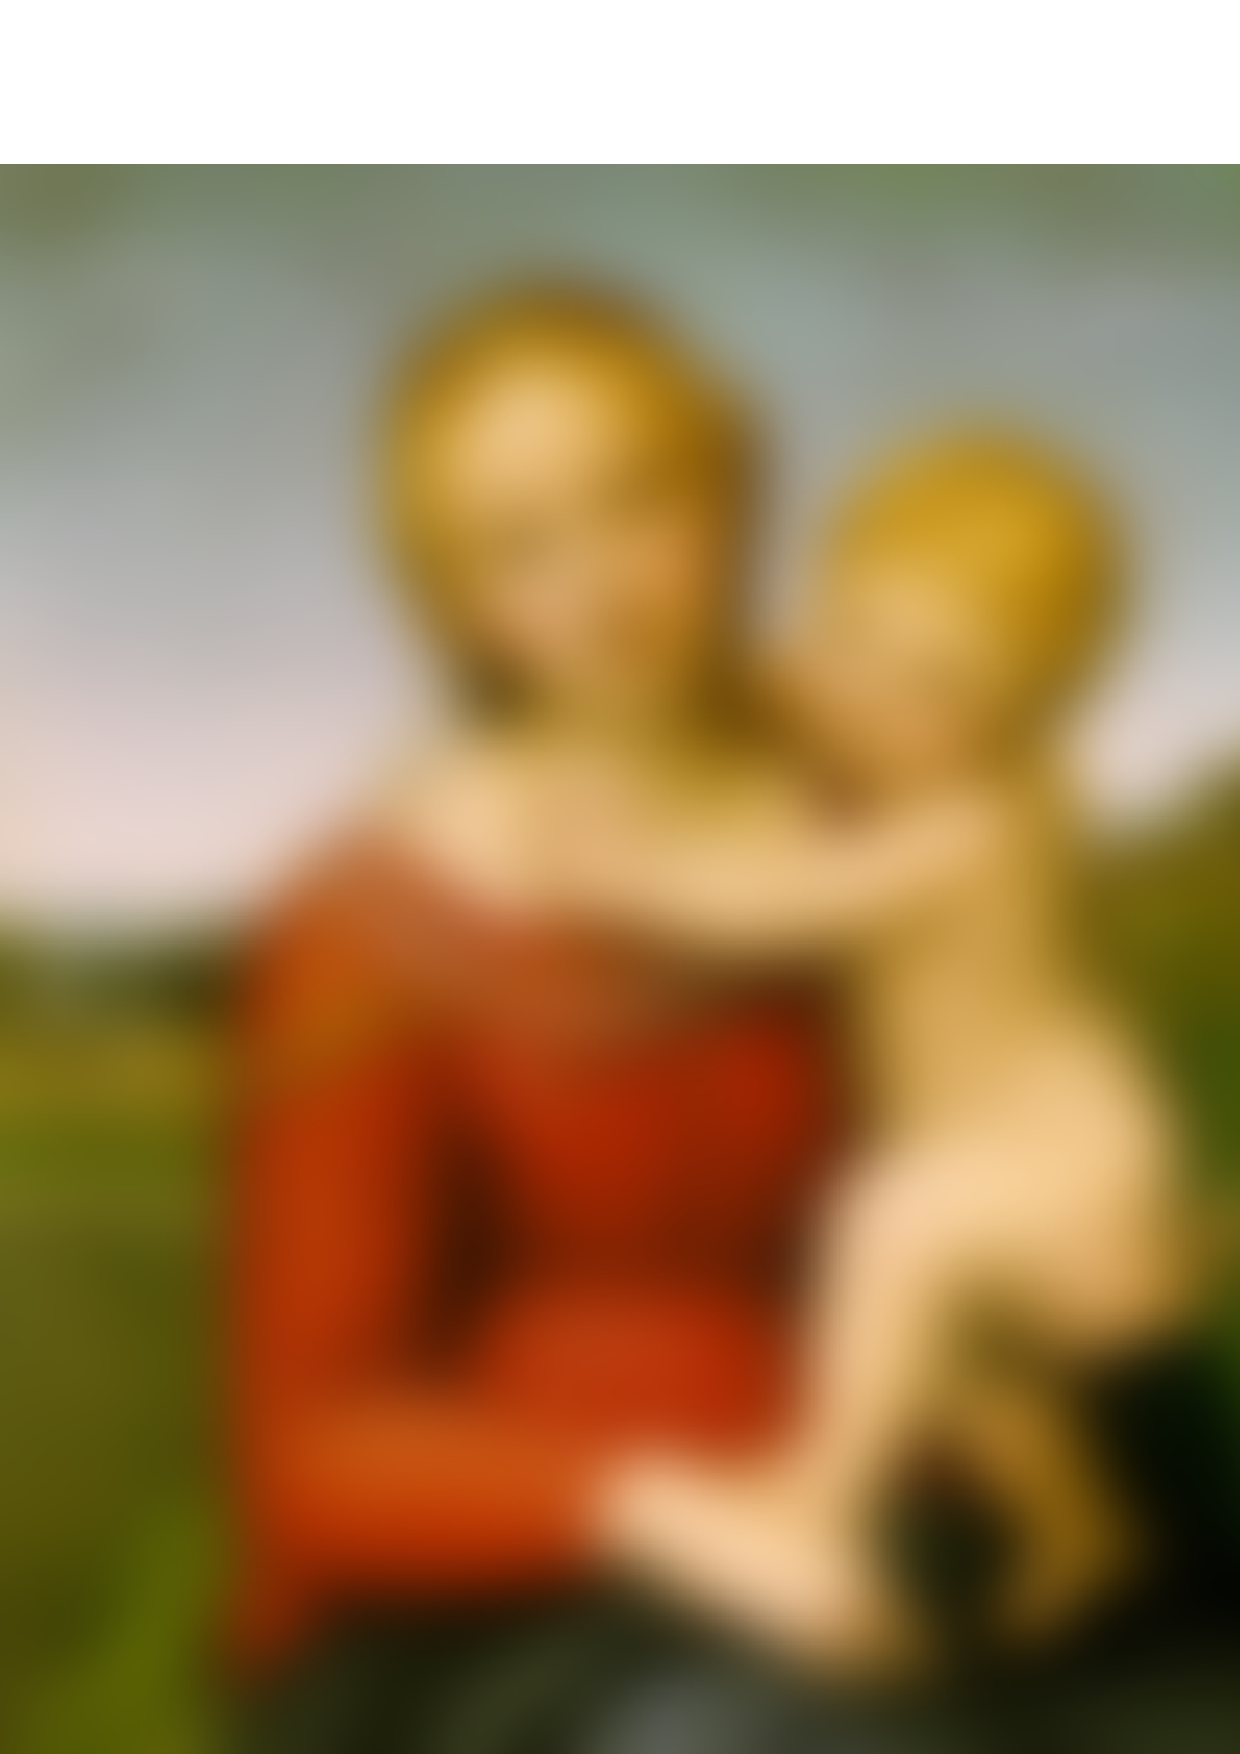
\includegraphics[width=\textwidth]{im1test.png}
    \caption{After the blurfilter with radius $r = 50$.}
  \end{subfigure}
  ~%
  \begin{subfigure}{0.3\textwidth}
    \includegraphics[width=\textwidth]{test.png}
    \caption{After the threshold filter.}
  \end{subfigure}
  \caption{Image result using the threshold filter and the blurfilter
    (with a radiues $r = 50$) on 
    \texttt{im1.png}. Before and after}
  \label{fig:thres}
\end{figure}
\message{ !name(report.tex) !offset(71) }

\end{document}

%%% Local Variables:
%%% mode: latex
%%% TeX-master: t
%%% End:
